\chapter{Background}
\label{chap:background}

The perplexing nature of human mind and intelligence has been a topic of many 
books, movies and shows. 
One would like to provide a coherent definition of intelligence, understand its 
emergence and measure it using a standardised scale.
The intelligence quotient (IQ) has been introduced as an attempt to quantify 
intelligence in terms of problem solving capabilities. 
Technological artifacts, whether computer programs or machines, have been 
equipped with artificial intelligence and successfully reproduced certain 
aspects of human behaviour in tasks such as chess playing \citep{ibmdeepblue} 
or simple psychotherapy \citep{Weizenbaum66}. However, these systems cannot 
exhibit the range of complex human behaviours which involve social 
interactions, learning and the ability to adapt to a new environment, to name a 
few. 
Recently, novel ways of looking at these problems emerged which emphasise the 
role of body and brain.
Embodiment has been recognised as fundamental to the understanding of natural 
and artificial intelligence \citep{Pfeifer2006}, while neuroscience attempts to 
identify the neural processes underlying cognition and intelligent behaviour.

\section{Brain, Body and Behaviour}
The way human intelligence emerges from brain processes and throughout the 
lifespan, as well as the way it is expressed continues to be a matter of 
debate. One way in which intelligence becomes apparent is through behaviour. 
Behaviour has been studied, measured and quantified within different approaches 
in psychology.
Behaviourism, which marked the first half of the twentieth century, aimed to 
systematically explain behaviour in response to environmental cues. Pavlov and 
Thorndike pioneered experimental research on animals and humans that analysed 
behaviour detached from the internal mental events. Behaviouristic theories 
emphasised the role of repetition, rewards and punishment in learning. These 
theories failed to explain some important factors in learning which influence 
human intelligence such as perception, language acquisition and comprehension. 
Moreover, they could not explain deviations in the behaviour due to 
the pathologies. Behaviourism was followed by the cognitive revolution which 
started in 1950s and tried to explain human behaviour in terms of underlying 
cognitive processes. Joint efforts to understand and mimic human cognition 
united researchers in psychology, anthropology, neuroscience, computer science 
and many others. Whereas behaviourism relied mostly on observable outcomes of 
experiments, the advent of the cognitive revolution introduced new methods and 
techniques to approach the analysis of mind. Those included psychophysical 
experiments, neuroimaging methods such as electroencephalography and the use of 
computers for simulations and modelling. Cognitivists viewed thought as a 
computation, where the brain operates on symbolic representations of the 
external 
world. They tried to identify and understand components of mental functions, 
and at the same time used these insights to create cognitive architectures that 
were supposed to incorporate learning, memory, language, reasoning and 
perception into artificial systems.
ACT-R \citep{Anderson1997} and SOAR \citep{Laird87} are examples of such 
architectures and they approximate cognitive processing by algorithms defined 
over internal representations of the external world.

The vast majority of theories and algorithms proposed in cognitivism were 
proven not to be feasible in creating artificial intelligence for several 
reasons. First, such algorithms had a very limited capacity to mimic cognitive 
processing as it occurs in the human brain because they could not reproduce the 
full spectrum of complex human behaviour. The way algorithms performed 
computations was lacking the link to the way the brain solves the same 
problems, 
making it hard to compare artificial with biological systems. 
Moreover, such algorithms frequently operated on preprocessed sensory data such 
as images or image excerpts that were acquired independently of constraints 
imposed by the body. In this way learning was not embedded into the environment 
which is a central aspect of human development. Finally, such approaches could 
not have been used to mimic even basic human abilities, such as perception, 
physical manipulation and speech \citep{Mingers01}. These points were the main 
criticism of the Good Old-Fashioned Artificial Intelligence, an approach which 
took a very exclusive view on intelligence by focusing on algorithms mimicking 
problem solving skills and logic inference.

The ideas within post-cognitivism that emerged at the end of the 20th century 
argued that mimicking human intelligence requires bodily agents in the world. 
Theories on embodied cognition emphasised the intertwined role of body and 
cognition since the way we think is largely influenced by our bodies 
\citep{LakoffJohnson80, varela06, plasticq}. Clark argued that 
biological brains are control systems for biological bodies and cognition is a 
situated activity because it operates in the context of task-relevant inputs 
and outputs. Because traditional view of cognition failed to explain how 
cognition interferes with perception and action, theories on grounded cognition 
gained a lot of attention among the proponents of embodied artificial 
intelligence. They proposed that knowledge is represented by modal 
representations and body imagery. For robotics, this means that simulations of 
sensorimotor experience could serve as computational mechanisms for the 
implementation of cognition in artificial agents.

The neuroscientific foundations of the human mind were also a matter of 
interest 
for scientists developing cognitive architectures.
They were expanded with neurobiologically plausible models 
that mimic neural activities (e.g. artificial neural networks). This is a first 
step towards simulating biological cognitive phenomena that could be compared 
to human brains. Only recently, large-scale brain simulations gained popularity 
among theorethical neuroscientists. Such models aim to provide explanations of 
brain processes through simulations of millions of artificial neurons. The 
Human Brain Project at EPFL in Switzerland aims to \emph{"answer age-old 
questions about how we think, remember, learn and feel``} \citep{Markram201139} 
by reverse engineering the human brain via thorough simulations of neural 
cellular mechanisms. The SPAUN brain model \citep{eliasmith_large-scale_2012} 
developed at the University of Waterloo in Canada uses simpler models of 
neurons to simulate human-like behaviour in a certain set of tasks. Although 
targeting different questions, both of these models 
have proven very powerful in replicating the data obtained in experiments with 
humans and animals. Lack of learning mechanisms and embodiment makes these 
models unsuitable for the study of the social and cognitive development. As 
many other neural and brain models, they assume fully developed systems 
omitting 
the role of growth and maturing. Disembodied models are also neglecting the 
role of interaction with the world and sensorimotor integration which are a 
crucial part of human development.

With this thesis, we explored the ground that involves these two aspects of 
cognition: embodied cognition and cognition emerging from simulated brain 
networks. A biologically inspired model for sensorimotor learning was developed 
and implemented on a humanoid robot. 


\section{Development of Social Cognition}
\label{sec:devsoccog}

Before stipulating the requirements needed to approach the analysis of social 
and cognitive skill development in artificial agents and neural models, we turn 
to what we know about human development. A large body of research in 
developmental psychology has focused on cognitive and social skill development 
in children. Jean Piaget pioneered the work by establishing the \emph{theory of 
cognitive development} which proposes four consecutive and universal stages of 
cognitive development: sensorimotor, preoperational, concrete operations and 
formal operations \citep{piaget73}. Piaget identified the age when these stages 
occur and he emphasised the role of children's exploratory behaviour in the 
environment. He postulated the importance of repetitive circular reactions in 
children which develop into more complex intentional actions. Piaget notes that 
the capability to coordinate sensorimotor actions is acquired during the first 
two years of infancy (e.g. through body babbling). 
Another developmental psychologist, Lev Vygotsky, constructed the 
\emph{sociocultural theory of development} which augments the theory proposed 
by Piaget by stating the importance of the social and cultural context in the 
cognitive development \citep{Vyg78}.
This role is evident in the support children receive through scaffolding by 
their caregivers. Vygotsky defines the \emph{zone of proximal development} as 
the gap between what a learner has already accomplished and what she or he can 
achieve only with guidance. This is to say that social interactions are a  
necessary part in the development of higher mental functions.
\newline
\phantom{x}\hspace{3ex} 
An important part of social interactions is the ability to understand and manipulate attentional behaviours. Attention is also required for many learning mechanisms, such as imitation learning \citep{Tomasello1995}. Joint attention is the ability of interacting individuals to share the focus of attention.
It is thus an essential part of the human development and an important topic in the study of human-robot interaction. Several motor and cognitive skills precede the development of joint attention: the ability to detect the focus of attention of the interacting partner, detection and maintenance of eye contact and manipulation of the focus of attention of the interacting partner \citep{Kaplan2006}. The manipulation of the focus of attention can be achieved through pointing gestures which in humans start early in infancy, around the age of nine months \citep{baron1997mindblindness}. At this stage, the primitive forms of pointing are known as imperative pointing. It is used as a request for a certain object and it may arise from failed reaching actions. Around the age of twelve months, pointing starts to 
become declarative and is used to draw the caregiver's attention to 
something which might also be out of reach for the adult.
In infants, it is assumed that pointing emerges from failed attempts of 
grasping movements towards an object \citep{Hafner2011}. Following the 
Vygotsky's view, when caregivers react to such behaviour by giving the object 
to the child, he or she starts to internalise such behaviour throughout 
multiple repetitions. Finally, this failed grasping attempts seem to acquire 
the meaning of a pointing gesture afterwards.
\newline
\phantom{x}\hspace{3ex} In this thesis, we take the approach of \emph{developmental} or 
\emph{epigenetic} robotics aiming to answer the question whether pointing 
emerges from grasping \citep{Kaplan2006}. This approach is concerned with motor 
and cognitive development in artificial systems and utilises knowledge about 
the development as it occurs in infants. We adhere to the developmental 
trajectory defined by Piaget and start with a simple self-exploration behaviour 
that eventually builds up to more complex behaviours such as the ability to 
share the focus of attention.  In the robotics literature, interesting studies 
can be found on the development of motor competences in artificial agents.
In \citep{Metta2000}, the author implemented on a humanoid robot an adaptive 
control system inspired by biological development of visuo-motor coordination 
for the acquisition of orienting and reaching behaviours. Following a 
developmental paradigm, the system starts with moving the eyes only. At this 
point, control is a mixture of random and goal-directed movements. The 
development proceeds with the acquisition of closed loop gains, reflex-like 
modules controlling the arm sub-system, acquisition of an eye-head coordination 
and of a head-arm coordination map. 
 
In \citep{Hafner2011}, the development of pointing behaviours in a humanoid 
robot has been addressed. In particular, a humanoid robot (Aldebaran Nao) has 
been programmed to acquire early motor competences through an exploration 
behaviour, namely body babbling. 
Learning consisted in the robot exploring its arm movements while collecting 
sensorimotor data (hand and arm joint positions), thus building up an internal 
model of its own body. A simple predictive algorithm provided the robot with a 
mechanism for producing motor commands to reach the desired hand positions. 
Pointing behaviours emerged when target points were presented outside the reach 
of the robot, thus strengthening the hypothesis that pointing may arise from 
grasping. The contribution of this thesis to the existing body of research in 
this field is to enrich models with algorithms that are inspired by the way 
the human brain deals with the same issue.

\section{Neuroscientific Perspective}
\label{sec:neurosci}

The theories on social and cognitive development successfully explain 
observable consequences of infants' behaviour. 
To understand the causes of the development in terms of changes in the brain, 
one has to investigate the underlying neural mechanisms. Finding a relation 
between neural processes and the behaviour may enrich our knowledge about the 
interplay between genetic and environmental factors, which remains a topic of 
debate in the developmental community. In addition, understanding neural 
underpinnings would help us explain the outcomes of different neural disorders 
and pathologies on behaviour. Finally, such information would be valuable for 
computational neuroscientists that aim to investigate development using 
biologically realistic systems.

\subsection{Brain Development}
\label{ssec:braindev}

\begin{figure}[ht]
\centering
%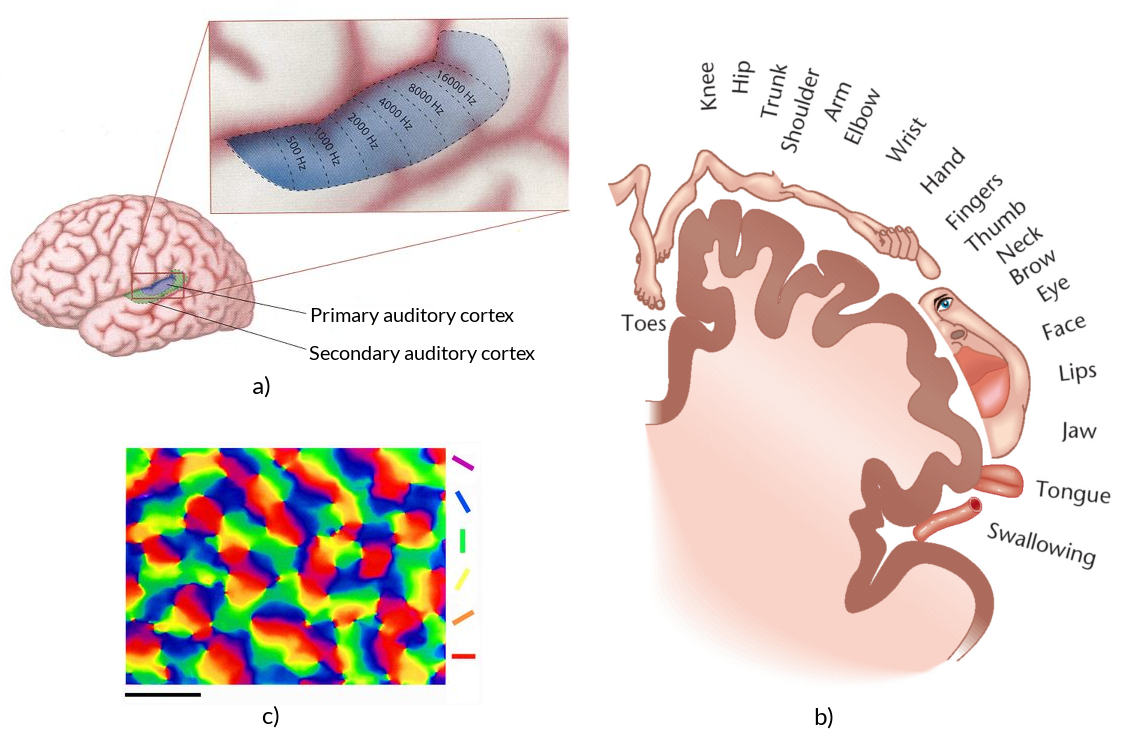
\epsfig{file=maps.png, height=10cm}
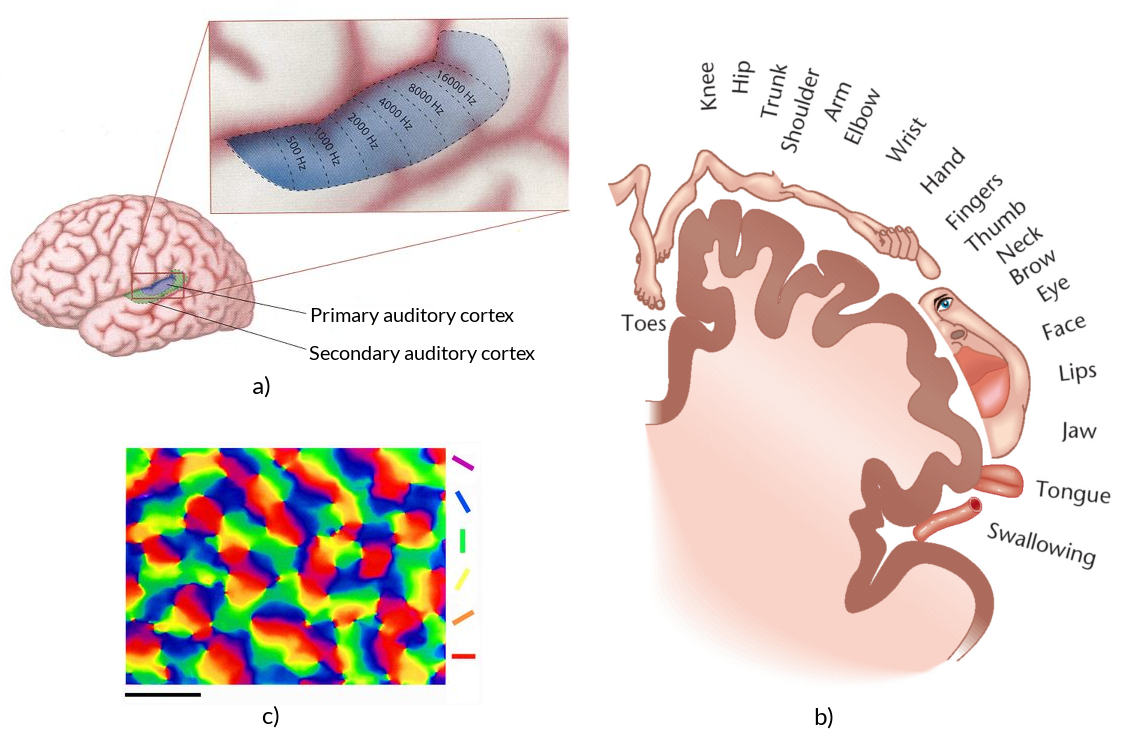
\includegraphics[scale=0.38]{maps.png}
\caption[Examples of topographic maps in the human brain]{Examples of
topographic maps in the human brain: cortical tonotopy (a), somatotopy (b) and 
orientation selectivity map (c). Images retrieved from: 
\url{
http://www.cns.nyu.edu/~david/courses/perception/lecturenotes/localization/loc 
alization-slides/Slide5.jpg}, \url{
http://images.scholarpedia.org/w/images/9/95/Visual_map_Swindale_Monkey_ori_doma
ins_Blasdel_1986.jpg}
and \url{http://spinacare.files.wordpress.com/2007/02/homunculus.jpg}}
\label{lab:tonotopy}
\end{figure}

The first years of an infant's brain development are characterised by stunning 
changes. By the age of three the brain has reached 80 percent of its adult 
volume \citep{SCI:Gil2007d, Nowakowski} and it has up to twice as 
many synapses as it will have in adulthood \citep{Krieg63}. Over time, in a 
process called \emph{synaptic pruning} redundant synapses are gradually 
discarded. The change in brain function and structure is known as \emph{brain 
plasticity} and is influenced by genetic and environmental factors. Greenough 
and Black \citep{GreenoughBlackWallace87} proposed a theory of two different 
types of brain plasticity: \emph{experience-expectant} (specific sensory 
experiences and input are needed at specific times for neural development and 
maturation) and \emph{experience-dependent} (interaction with the environment 
to develop skills for later use). The experience-dependent brain plasticity 
complies with the Vygotsky's theory on social development. Because genetic 
instructions are not sufficient to 
specify neural connections with sufficient precision, additional brain 
principles contribute to neural plasticity \citep{singer86}. One of these 
principles is \emph{self-organisation} which allows to optimise genetically 
determined blue prints of connectivity by shaping the structural and functional 
role of brain areas according to the sensory input. 
\newline
\phantom{x}\hspace{3ex} Here, we focus on the way sensory information is 
organised in the brain and analyse the influence of self-organisation. Sensory 
input to the human brain is often organised in the topographic structure. This 
means that adjacent brain regions process sensory inputs with similar features. 
Such regions are known as \emph{sensory maps}. Sensory maps in the human brain 
contain neurons specialised in encoding specific modalities of sensory input. 
The plasticity in these areas is driven by the gradual formation of internal 
representations across the lifespan \citep{helgeritter1990, ph2013development}. 
Tonotopic organization is a spatial arrangement in the auditory cortex where 
similar frequencies are processed by neighbouring brain regions. Orientation 
maps recorded in the visual cortex contain pinwheel formations where neurons 
exhibiting highest activities for certain orientations in the visual input are 
spatially grouped together. Finally, there are somatotopic maps such as 
the cortical homunculus that approximate cortical areas representing different 
body parts. All three maps are shown in Figure \ref{lab:tonotopy}. Neurons in 
that region show interesting \emph{self-organising} properties - if a part of 
the 
body is amputated, the neural correlate of that part will be ``overtaken'' by 
the neighbouring tissue increasing the sensation of the body part represented 
through that tissue. Merzenich \citep{merzenich:amputation} showed the 
reorganisation of cortical maps 
in monkeys before and after the amputation of fingers. This type of functional 
plasticity is known as cortical re-mapping.
The self-organising property also becomes evident in sensory maps throughout 
brain development. For example, Farah \citep{Farah98} argues that 
self-organization in somatosensory maps takes place in the womb while the pose 
of the foetus imposes mutual touching of the face and the hands, as well as the 
feet and the genitals. She proposes that this might be the reason why these 
body parts, although not close to each other physically, are represented close 
to each other in the brain. 

\subsection{Challenges in Modelling of Brain Development}
Unraveling neural mechanisms in a developing brain of a person acting in the 
environment is a very complex task due to several reasons. First, one would 
need to record brain activity over a sustained period of time where development 
occurs. Most current brain imaging techniques require a controlled setting that 
is hard to introduce as a part of everyday routine.
To record from brains of infants and young children, they should continuously 
participate in such experiments. Apart from dedicated involvement, there is a 
danger that in such a setting they might not behave spontaneously as they would 
when exposed to their usual environment. Second, it needs to be defined what 
level of brain activity should be recorded (i.e. smaller populations of neurons 
vs. brain areas), and how to relate anatomical and functional changes of a 
developing brain within the social and cultural context. Developmental robotics 
in combination with biologically realistic brain models might help set the 
ground for this investigation. Robots equipped with artificial neural networks 
that capture ongoing development provide a controlled environment 
to analyse and steer learning mechanisms infants might employ when interacting 
with humans. 
%In this way, investigation of a developing brain might be more feasible based 
%on cues obtained via experiments with robots. 

In this thesis, the knowledge about the developing brain from studies 
with animals, as well as lesion studies in human brains, has been utilised to 
develop a computational model based on artificial neural networks.
Two properties of the developing brain, self-organisation and topology 
preservation, have been phenomenologically captured using the model.
Implementation of the model on a robotic platform accounts for a realistic 
sensory experience, that might simulate those of a small child throughout the 
early stages of development. 
